\chapter{Biosíntesis y célula integrada}\label{ch:b1:biosyntheses-integration}

A las ocho de la mañana un hígado convierte el azúcar del desayuno en
\omterm{def:b1:carbohydrates:polysaccharide}{glucógeno} y en \omterm{def:b1:lipids:triglyceride}{grasa}; a las tres de la madrugada siguiente ese mismo hígado
fabrica azúcar a partir de los \omterm{def:b1:proteins:aminoacid}{aminoácidos} del músculo y lo vierte a la
sangre para un encéfalo que lleva nueve horas sin comer. Nada ha cambiado en
las \omterm{def:b1:enzymes:enzyme}{enzimas}; lo que ha cambiado es cuáles de ellas están encendidas. Los
capítulos anteriores desmontaron las moléculas de la \omterm{def:b1:cell-unit-of-life:cell}{célula}; este las monta
--- las síntesis de azúcares, \omterm{def:b1:carbohydrates:polysaccharide}{glucógeno}, \omterm{def:b1:lipids:triglyceride}{grasas} y \omterm{def:b1:proteins:aminoacid}{aminoácidos} --- y se
pregunta después cómo deciden una \omterm{def:b1:cell-unit-of-life:cell}{célula}, y un \omterm{def:b1:organism-environment:organism}{organismo}, qué vías funcionan
en cada momento. La respuesta es un pequeño conjunto de monedas comunes,
unas pocas \omterm{def:b1:enzymes:enzyme}{enzimas} en las encrucijadas, y hormonas que informan a todas las
\omterm{def:b1:cell-unit-of-life:cell}{células} del estado del conjunto.

\section{Qué necesita una síntesis}

\begin{proposition}[Los tres requisitos del anabolismo]\label{prop:b1:biosyntheses-integration:needs}
\index{anabolismo}
Toda biosíntesis necesita \emph{esqueletos carbonados}, tomados de un puñado
de intermediarios de la \omterm{def:b1:respiration-fermentation:glycolysis}{glucólisis} y del \omterm{def:b1:respiration-fermentation:krebs}{ciclo de Krebs}; \emph{poder
reductor}, suministrado como \omterm{def:b1:biosyntheses-integration:ppp}{NADPH}; y \emph{energía}, suministrada como \omterm{def:b1:water-small-molecules:atp}{ATP}.
El catabolismo y el anabolismo se encuentran, pues, en las mismas
encrucijadas --- glucosa-6-fosfato, triosa fosfato, piruvato, \omterm{def:b1:respiration-fermentation:pdh}{acetil-CoA},
$\alpha$-cetoglutarato, oxalacetato ---, pero funcionan con \omterm{def:b1:enzymes:enzyme}{enzimas}
separadas en los pasos irreversibles, de modo que cada sentido puede
encenderse de forma independiente, y usan \omterm{def:b1:enzymes:enzyme}{coenzimas} distintas para sus
electrones: el NADH, mantenido oxidado, para retirar electrones en el
catabolismo; el \omterm{def:b1:biosyntheses-integration:ppp}{NADPH}, mantenido reducido, para cederlos en la síntesis.
\end{proposition}

\begin{definition}[La vía de las pentosas fosfato]\label{def:b1:biosyntheses-integration:ppp}
\index{vía de las pentosas fosfato}\index{NADPH}
La \emph{vía de las pentosas fosfato} del \omterm{def:b1:eukaryotic-cell:organelle}{citosol} oxida la
glucosa-6-fosfato a ribulosa-5-fosfato y $\mathrm{CO_2}$, y reduce dos
$\mathrm{NADP^+}$ a NADPH; su rama no oxidativa interconvierte después
azúcares fosforilados de cinco, cuatro, seis y siete carbonos, de modo que
la \omterm{def:b1:cell-unit-of-life:cell}{célula} puede fabricar ribosa-5-fosfato para los \omterm{def:b1:nucleic-acids:nucleotide}{nucleótidos} cuando
necesita pentosas, NADPH cuando necesita poder reductor (síntesis de \omterm{def:b1:lipids:triglyceride}{grasas},
defensa frente a oxidantes) o ambas cosas, y devolver el resto a la
\omterm{def:b1:respiration-fermentation:glycolysis}{glucólisis}. Es la fuente principal de NADPH en las \omterm{def:b1:cell-unit-of-life:cell}{células} animales; en las
plantas, las \omterm{prop:b1:photosynthesis:lightreactions}{reacciones luminosas} del cloroplasto suministran NADPH de día.
\end{definition}

\begin{omfigure}
\begin{tikzpicture}[font=\footnotesize, >=Stealth, line cap=round,
  hub/.style={draw, thick, rounded corners=3pt, fill=omDef!12, inner sep=3pt, align=center},
  prod/.style={draw, thick, rounded corners=3pt, fill=omExo!15, inner sep=3pt, align=center},
  fuel/.style={draw, thick, rounded corners=3pt, fill=omProp!15, inner sep=3pt, align=center}]
  \node[hub] (g6p) at (0,4.5) {glucosa-6-P};
  \node[hub] (tp) at (0,2.8) {triosa-P};
  \node[hub] (pyr) at (0,1.1) {piruvato};
  \node[hub] (accoa) at (0,-0.6) {acetil-CoA};
  \node[hub] (krebs) at (0,-2.4) {ciclo de Krebs\\ ($\alpha$-CG, OAA)};
  \draw[<->, thick] (g6p) -- (tp); \draw[<->, thick] (tp) -- (pyr); \draw[->, thick] (pyr) -- (accoa); \draw[->, thick] (accoa) -- (krebs);
  % left: stores and fuels in
  \node[fuel] (gly) at (-4.2,4.5) {glucógeno, almidón}; \draw[<->, thick] (gly) -- (g6p);
  \node[fuel] (lac) at (-4.2,1.1) {lactato}; \draw[<->, thick] (lac) -- (pyr);
  \node[fuel] (fa) at (-4.2,-0.6) {ácidos grasos}; \draw[<->, thick] (fa) -- (accoa) node[pos=0.62, below=2pt, font=\scriptsize] {$\beta$-oxidación / síntesis};
  \node[fuel] (aa) at (-4.2,-2.4) {aminoácidos}; \draw[<->, thick] (aa) -- (krebs) node[pos=0.4, below=2pt, font=\scriptsize] {transaminación};
  % right: products
  \node[prod] (ppp) at (4.3,4.5) {vía de las pentosas fosfato:\\ NADPH, ribosa-5-P $\to$ nucleótidos}; \draw[->, thick] (g6p) -- (ppp);
  \node[prod] (glyc) at (4.3,2.8) {glicerol $\to$ lípidos}; \draw[->, thick] (tp) -- (glyc);
  \node[prod] (ala) at (4.3,1.1) {alanina, serina, glicina}; \draw[<->, thick] (pyr) -- (ala);
  \node[prod] (chol) at (4.3,-0.6) {colesterol, esteroides;\\ cuerpos cetónicos}; \draw[->, thick] (accoa) -- (chol);
  \node[prod] (glu) at (4.3,-2.4) {glutamato, aspartato\\ y sus familias; hemo}; \draw[<->, thick] (krebs) -- (glu);
  \draw[->, very thick, omThm] (1.4,-2.0) -- (1.4,0.65) node[pos=0.5, rotate=90, anchor=south, font=\scriptsize, omThm] {gluconeogénesis};
\end{tikzpicture}

{\small Las encrucijadas del metabolismo. Seis \omterm{def:b1:flowering-plant-organization:organs}{nudos} de las vías centrales
(azul) reciben combustibles y reservas (naranja) y abastecen todas las
biosíntesis (verde). La \omterm{def:b1:biosyntheses-integration:gluconeogenesis}{gluconeogénesis} (rojo) recorre hacia arriba el
centro del mapa.}
\end{omfigure}

\section{Fabricar glucosa: la gluconeogénesis}

\begin{definition}[Gluconeogénesis]\label{def:b1:biosyntheses-integration:gluconeogenesis}
\index{gluconeogénesis}
La \emph{gluconeogénesis} fabrica glucosa a partir de precursores no
glucídicos --- lactato, piruvato, glicerol y los esqueletos carbonados de
casi todos los \omterm{def:b1:proteins:aminoacid}{aminoácidos} --- en el hígado (y algo en el riñón). Recorre la
\omterm{def:b1:respiration-fermentation:glycolysis}{glucólisis} al revés en sus siete pasos reversibles y esquiva los tres
irreversibles con \omterm{def:b1:enzymes:enzyme}{enzimas} distintas: el piruvato se carboxila a oxalacetato
(en la \omterm{def:b1:eukaryotic-cell:mitochondrion}{mitocondria}, un \omterm{def:b1:water-small-molecules:atp}{ATP}) y se descarboxila a fosfoenolpiruvato (un GTP);
la fructosa-1,6-bisfosfato se hidroliza a fructosa-6-fosfato; y la
glucosa-6-fosfato se hidroliza a glucosa libre, que sale de la \omterm{def:b1:cell-unit-of-life:cell}{célula}. Por
glucosa: 6 equivalentes de \omterm{def:b1:water-small-molecules:atp}{ATP} y 2 NADH, frente a los 2 \omterm{def:b1:water-small-molecules:atp}{ATP} que rinde la
\omterm{def:b1:respiration-fermentation:glycolysis}{glucólisis}: el precio de recorrer cuesta arriba un camino cuesta abajo.
\end{definition}

\begin{omfigure}
\begin{tikzpicture}[font=\footnotesize, >=Stealth, line cap=round,
  m/.style={draw, thick, rounded corners=3pt, inner sep=3pt, fill=omDef!10, align=center}]
  \node[m] (glc) at (0,5.2) {glucosa};
  \node[m] (g6p) at (0,3.9) {glucosa-6-P};
  \node[m] (f6p) at (0,2.6) {fructosa-6-P};
  \node[m] (fbp) at (0,1.3) {fructosa-1,6-bisP};
  \node[m] (pep) at (0,-0.5) {fosfoenolpiruvato};
  \node[m] (pyr) at (0,-1.9) {piruvato};
  \node[m] (oaa) at (5.2,-1.9) {oxalacetato};
  % glycolysis (down, left side)
  \draw[->, thick, omDef!70!black] (glc.west) ++(-0.2,0) -- ++(-1.0,0) |- (g6p.west) node[pos=0.25, left, font=\scriptsize, align=right] {hexoquinasa\\ ATP};
  \draw[->, thick, omDef!70!black] (f6p.west) ++(-0.2,0) -- ++(-1.0,0) |- (fbp.west) node[pos=0.25, left, font=\scriptsize, align=right] {PFK\\ ATP};
  \draw[->, thick, omDef!70!black] (pep.west) ++(-0.2,0) -- ++(-1.0,0) |- (pyr.west) node[pos=0.25, left, font=\scriptsize, align=right] {piruvato quinasa\\ ATP producido};
  \draw[<->, thick] (g6p) -- (f6p); \draw[<->, thick] (fbp) -- (pep) node[midway, right, font=\scriptsize] {pasos reversibles (comunes)};
  % gluconeogenesis (up, right side)
  \draw[->, thick, omThm] (g6p.east) ++(0.2,0) -- ++(1.0,0) |- (glc.east) node[pos=0.25, right, font=\scriptsize, align=left] {glucosa-6-fosfatasa\\ (solo hígado)};
  \draw[->, thick, omThm] (fbp.east) ++(0.2,0) -- ++(1.0,0) |- (f6p.east) node[pos=0.25, right, font=\scriptsize, align=left] {fructosa-1,6-\\ bisfosfatasa};
  \draw[->, thick, omThm] (pyr) -- (oaa) node[midway, below=3pt, font=\scriptsize] {piruvato carboxilasa, ATP};
  \draw[->, thick, omThm] (oaa) |- (pep.east);
  \node[anchor=south, font=\scriptsize, omThm] at (3.6,-0.4) {PEP carboxiquinasa, GTP};
  \node[anchor=north, align=center, gray] at (1.0,-2.7) {azul: glucólisis (hacia abajo); rojo: los tres desvíos de la gluconeogénesis (hacia arriba)\\ coste de una glucosa a partir de dos piruvatos: 4 ATP $+$ 2 GTP $+$ 2 NADH};
\end{tikzpicture}

{\small La \omterm{def:b1:respiration-fermentation:glycolysis}{glucólisis} y la \omterm{def:b1:biosyntheses-integration:gluconeogenesis}{gluconeogénesis} comparten siete reacciones
reversibles y difieren en tres irreversibles, cada una esquivada por una
\omterm{def:b1:enzymes:enzyme}{enzima} distinta. \omterm{def:b1:enzymes:enzyme}{Enzimas} distintas significan controles distintos: el hígado
puede encender un sentido y apagar el otro.}
\end{omfigure}

\begin{proposition}[Qué puede y qué no puede convertirse en glucosa]\label{prop:b1:biosyntheses-integration:cannot}
El lactato, el glicerol y los \omterm{def:b1:proteins:aminoacid}{aminoácidos} que rinden piruvato o
intermediarios del \omterm{def:b1:respiration-fermentation:krebs}{ciclo de Krebs} (todos menos la leucina y la lisina)
pueden convertirse en glucosa. Los \omterm{def:b1:lipids:fattyacid}{ácidos grasos} no, en los animales: su
$\beta$-oxidación da \omterm{def:b1:respiration-fermentation:pdh}{acetil-CoA}, cuyos dos carbonos entran en el ciclo y
salen como dos $\mathrm{CO_2}$ antes de que se gane ningún oxalacetato, de
modo que no hay ruta neta del \omterm{def:b1:respiration-fermentation:pdh}{acetil-CoA} al azúcar. Las plantas, los hongos
y las bacterias poseen el \emph{ciclo del glioxilato}, un atajo que se salta
las dos descarboxilaciones y permite a una semilla oleaginosa en germinación
convertir su \omterm{def:b1:lipids:triglyceride}{grasa} en el azúcar que necesita su plántula. Un mamífero que
pasa hambre, en cambio, debe fabricar su glucosa a partir de \omterm{def:b1:proteins:peptide}{proteínas}.
\end{proposition}

\begin{example}[El ciclo de Cori]\label{ex:b1:biosyntheses-integration:cori}
Un músculo que esprinta fermenta \omterm{def:b1:carbohydrates:polysaccharide}{glucógeno} a lactato, que pasa a la sangre;
el hígado capta el lactato, lo oxida a piruvato, fabrica glucosa a partir de
él a 6 \omterm{def:b1:water-small-molecules:atp}{ATP} por glucosa y devuelve la glucosa a la sangre para que el músculo
vuelva a usarla. El músculo ha ganado 2 \omterm{def:b1:water-small-molecules:atp}{ATP} por glucosa sin oxígeno y le ha
pasado al hígado una factura de 6, que este paga con oxígeno y sin prisa: la
``deuda de oxígeno'' de un esprint se salda en buena parte en el hígado.
\end{example}

\section{Almacenar: glucógeno y grasa}

\begin{definition}[Síntesis de glucógeno]\label{def:b1:biosyntheses-integration:glycogensynthesis}
La glucosa se almacena como \omterm{def:b1:carbohydrates:polysaccharide}{glucógeno} activando la glucosa-6-fosfato a
\emph{UDP-glucosa} (un UTP), que la \emph{\omterm{def:b1:carbohydrates:polysaccharide}{glucógeno} sintasa} añade a los
extremos no reductores del árbol ya existente; una \emph{\omterm{def:b1:enzymes:enzyme}{enzima} ramificante}
corta y vuelve a unir cadenas cortas para formar las ramificaciones
$\alpha(1{\to}6)$ (\cref{ch:b1:carbohydrates}). La sintasa y la fosforilasa
se regulan en sentidos opuestos por las mismas señales: la fosforilación que
enciende la fosforilasa apaga la sintasa, de modo que el árbol nunca se
construye y se desmonta a la vez.
\end{definition}

\begin{definition}[Síntesis de ácidos grasos]\label{def:b1:biosyntheses-integration:fasynthesis}
\index{síntesis de ácidos grasos}
Los \omterm{def:b1:lipids:fattyacid}{ácidos grasos} se fabrican en el \omterm{def:b1:eukaryotic-cell:organelle}{citosol} a partir del \omterm{def:b1:respiration-fermentation:pdh}{acetil-CoA}
exportado desde la \omterm{def:b1:eukaryotic-cell:mitochondrion}{mitocondria}. La \emph{\omterm{def:b1:respiration-fermentation:pdh}{acetil-CoA} carboxilasa}, el paso
regulado, lo carboxila (un \omterm{def:b1:water-small-molecules:atp}{ATP}) a malonil-CoA; la \emph{\omterm{def:b1:lipids:fattyacid}{ácido graso} sintasa}
añade después dos carbonos cada vez desde el malonil-CoA a una cadena en
crecimiento, y reduce cada adición con dos \omterm{def:b1:biosyntheses-integration:ppp}{NADPH}, hasta que se libera el
palmitato (C16): 8 \omterm{def:b1:respiration-fermentation:pdh}{acetil-CoA}, 7 \omterm{def:b1:water-small-molecules:atp}{ATP} y 14 \omterm{def:b1:biosyntheses-integration:ppp}{NADPH} por palmitato. La
elongación y la desaturación en el \omterm{def:b1:eukaryotic-cell:endomembrane}{retículo endoplasmático} fabrican los
demás ácidos; la esterificación con glicerol-3-fosfato (procedente de la
triosa fosfato) fabrica los \omterm{def:b1:lipids:triglyceride}{triglicéridos}. La vía no es la
$\beta$-oxidación al revés: \omterm{def:b1:enzymes:enzyme}{enzimas} distintas, compartimento distinto,
malonil-CoA en vez de \omterm{def:b1:respiration-fermentation:pdh}{acetil-CoA}, \omterm{def:b1:biosyntheses-integration:ppp}{NADPH} en vez de $\mathrm{FADH_2}$ y NADH;
y el malonil-CoA bloquea el transporte de \omterm{def:b1:lipids:fattyacid}{ácidos grasos} al interior de la
\omterm{def:b1:eukaryotic-cell:mitochondrion}{mitocondria}, de modo que una \omterm{def:b1:cell-unit-of-life:cell}{célula} no fabrica \omterm{def:b1:lipids:triglyceride}{grasa} y la quema a la vez.
\end{definition}

\begin{example}[Grasa a partir de azúcar]\label{ex:b1:biosyntheses-integration:fatfromsugar}
Un hígado al que se da más glucosa de la que puede almacenar como \omterm{def:b1:carbohydrates:polysaccharide}{glucógeno}
fabrica \omterm{def:b1:lipids:triglyceride}{grasa}: glucosa a piruvato y a \omterm{def:b1:respiration-fermentation:pdh}{acetil-CoA} (con pérdida de un tercio
del carbono como $\mathrm{CO_2}$ y ganancia de \omterm{def:b1:water-small-molecules:atp}{ATP}), \omterm{def:b1:respiration-fermentation:pdh}{acetil-CoA} a palmitato
a costa de ese \omterm{def:b1:water-small-molecules:atp}{ATP} y del \omterm{def:b1:biosyntheses-integration:ppp}{NADPH} de la \omterm{def:b1:biosyntheses-integration:ppp}{vía de las pentosas fosfato}, y
palmitato a \omterm{def:b1:lipids:triglyceride}{triglicérido} enviado al \omterm{def:b1:body-plans-tissues:tissue}{tejido} adiposo. Alrededor del
\qty{15}{\%} de la energía del azúcar se pierde en la conversión; el resto
se almacena nueve veces más compacto que como \omterm{def:b1:carbohydrates:polysaccharide}{glucógeno}
(\cref{ch:b1:lipids}). Lo contrario --- \omterm{def:b1:lipids:triglyceride}{grasa} a azúcar --- es imposible.
\end{example}

\section{Nitrógeno: aminoácidos y nucleótidos}

\begin{definition}[Asimilación del nitrógeno, transaminación]\label{def:b1:biosyntheses-integration:nitrogen}
\index{transaminación}\index{glutamato}
El amonio entra en la materia orgánica casi por completo a través del
\emph{glutamato}: la glutamato deshidrogenasa lo añade al
$\alpha$-cetoglutarato, y la glutamina sintetasa añade un segundo a la
\omterm{def:b1:proteins:aminoacid}{cadena lateral} del glutamato (un \omterm{def:b1:water-small-molecules:atp}{ATP}) y forma glutamina. A partir de esos
dos donantes, las \emph{transaminasas} (aminotransferasas, con una \omterm{def:b1:enzymes:enzyme}{coenzima}
derivada de la vitamina B$_6$) trasladan el grupo amino a cualquier
$\alpha$-cetoácido y construyen \omterm{def:b1:proteins:aminoacid}{aminoácidos} con los esqueletos carbonados de
las vías centrales: la familia del glutamato a partir del
$\alpha$-cetoglutarato, la familia del aspartato a partir del oxalacetato, y
la alanina y la serina a partir del piruvato y del 3-fosfoglicerato. Las
plantas y las bacterias fabrican los veinte; los animales han perdido las
vías largas de nueve de ellos, los \omterm{def:b1:proteins:aminoacid}{aminoácidos} \emph{esenciales}, y los
toman del alimento. Esas mismas transaminasas, al revés, arrancan el
nitrógeno de los \omterm{def:b1:proteins:aminoacid}{aminoácidos} sobrantes para excretarlo como amoniaco (peces),
urea (mamíferos) o ácido úrico (aves, insectos).
\end{definition}

\begin{example}[Nucleótidos]\label{ex:b1:biosyntheses-integration:nucleotides}
Un anillo de \omterm{def:b1:nucleic-acids:nucleotide}{purina} se ensambla sobre la ribosa-5-fosfato a partir de
glicina, aspartato, dos glutaminas, dos unidades de un carbono y
$\mathrm{CO_2}$, a un coste de seis \omterm{def:b1:water-small-molecules:atp}{ATP}; una \omterm{def:b1:nucleic-acids:nucleotide}{pirimidina}, a partir de
aspartato y de carbamoil fosfato. Los desoxinucleótidos se fabrican a partir
de ribonucleótidos reduciendo el azúcar, con \omterm{def:b1:biosyntheses-integration:ppp}{NADPH}. Una \omterm{def:b1:cell-unit-of-life:cell}{célula} a punto de
dividirse fabrica unos $10^{10}$ \omterm{def:b1:nucleic-acids:nucleotide}{nucleótidos} en una hora; los fármacos que
bloquean estas síntesis --- el metotrexato, el 5-fluorouracilo --- detienen
primero las \omterm{def:b1:cell-unit-of-life:cell}{células} que se dividen, y por eso tratan el cáncer.
\end{example}

\section{El mamífero integrado}

\begin{proposition}[Alimentado y en ayunas]\label{prop:b1:biosyntheses-integration:fedfasting}
\index{insulina}\index{glucagón}
Los \omterm{def:b1:mammal-organization:organ}{órganos} se reparten el trabajo. Tras una comida, la \emph{insulina} del
páncreas ordena al hígado almacenar glucosa como \omterm{def:b1:carbohydrates:polysaccharide}{glucógeno} y convertir el
excedente en \omterm{def:b1:lipids:triglyceride}{grasa}, a los músculos captar glucosa y almacenar \omterm{def:b1:carbohydrates:polysaccharide}{glucógeno}, y
al \omterm{def:b1:body-plans-tissues:tissue}{tejido} adiposo captar \omterm{def:b1:lipids:triglyceride}{grasa}; la glucemia, que había subido a
\qty{8}{mmol/L}, vuelve a \qty{5}{} en dos horas. Entre comidas, el
\emph{glucagón} ordena al hígado degradar su \omterm{def:b1:carbohydrates:polysaccharide}{glucógeno} y, a medida que este
se agota, fabricar glucosa a partir de lactato, glicerol y \omterm{def:b1:proteins:aminoacid}{aminoácidos}, y al
\omterm{def:b1:body-plans-tissues:tissue}{tejido} adiposo liberar \omterm{def:b1:lipids:fattyacid}{ácidos grasos}, que los músculos y el hígado queman en
lugar de glucosa; el encéfalo, que no puede quemar \omterm{def:b1:lipids:triglyceride}{grasa}, conserva sus
\qty{120}{g} de glucosa al día. En un ayuno de varios días el hígado
convierte los \omterm{def:b1:lipids:fattyacid}{ácidos grasos} en \emph{cuerpos cetónicos}, ácidos pequeños que
el encéfalo puede usar, y la demanda de glucosa --- y de la \omterm{def:b1:proteins:peptide}{proteína} que la
produce --- cae en dos tercios. Los mecanismos hormonales corresponden al
volumen del segundo año; la lógica metabólica es la de este capítulo.
\end{proposition}

\begin{omfigure}
\begin{tikzpicture}
\begin{axis}[
  width=0.9\linewidth, height=6.4cm,
  axis x line=bottom, axis y line=left,
  xmin=0, xmax=24, ymin=0, ymax=10.8,
  xlabel={hora del día (h)}, ylabel={glucemia (\unit{mmol/L})},
  xlabel style={font=\small, at={(axis description cs:0.5,-0.12)}, anchor=north},
  ylabel style={font=\small},
  tick label style={font=\small}, xtick={0,4,8,12,16,20,24}, ytick={0,2,4,6,8,10},
  clip=false,
]
\addplot[very thick, omDef, smooth] coordinates {(0,4.8) (4,4.6) (7,4.5) (8,7.5) (9,7.0) (10,5.5) (11,5.0) (12,4.9) (13,7.8) (14,6.8) (15,5.4) (16,5.0) (18,4.9) (19.5,7.6) (20.5,6.9) (22,5.4) (24,4.8)};
\draw[thick, omProp] (axis cs:7.5,0) -- (axis cs:7.5,0.5); \draw[thick, omProp] (axis cs:12.5,0) -- (axis cs:12.5,0.5); \draw[thick, omProp] (axis cs:19,0) -- (axis cs:19,0.5);
\node[font=\scriptsize, omProp, anchor=south] at (axis cs:7.5,0.55) {comida};
\node[font=\scriptsize, omProp, anchor=south] at (axis cs:12.5,0.55) {comida};
\node[font=\scriptsize, omProp, anchor=south] at (axis cs:19,0.55) {comida};
\fill[omExo!25] (axis cs:8,8.6) rectangle (axis cs:11,9.4); \node[font=\scriptsize, anchor=south] at (axis cs:9.5,9.5) {insulina: almacenar};
\fill[omThm!20] (axis cs:0,8.6) rectangle (axis cs:7,9.4); \node[font=\scriptsize, anchor=south] at (axis cs:3.5,9.5) {glucagón: el hígado libera};
\fill[omThm!20] (axis cs:22,8.6) rectangle (axis cs:24,9.4);
\draw[dashed, gray] (axis cs:0,5) -- (axis cs:24,5);
\end{axis}
\end{tikzpicture}

{\small La glucemia a lo largo de un día. Cada comida la eleva durante dos
horas mientras la insulina impulsa el almacenamiento; entre comidas y
durante la noche, el glucagón la mantiene cerca de \qty{5}{mmol/L} con el
\omterm{def:b1:carbohydrates:polysaccharide}{glucógeno} del hígado y la \omterm{def:b1:biosyntheses-integration:gluconeogenesis}{gluconeogénesis}. El \omterm{def:b1:organism-environment:homeostasis}{valor de consigna} se sostiene
dentro de un factor dos.}
\end{omfigure}

\begin{omfigure}
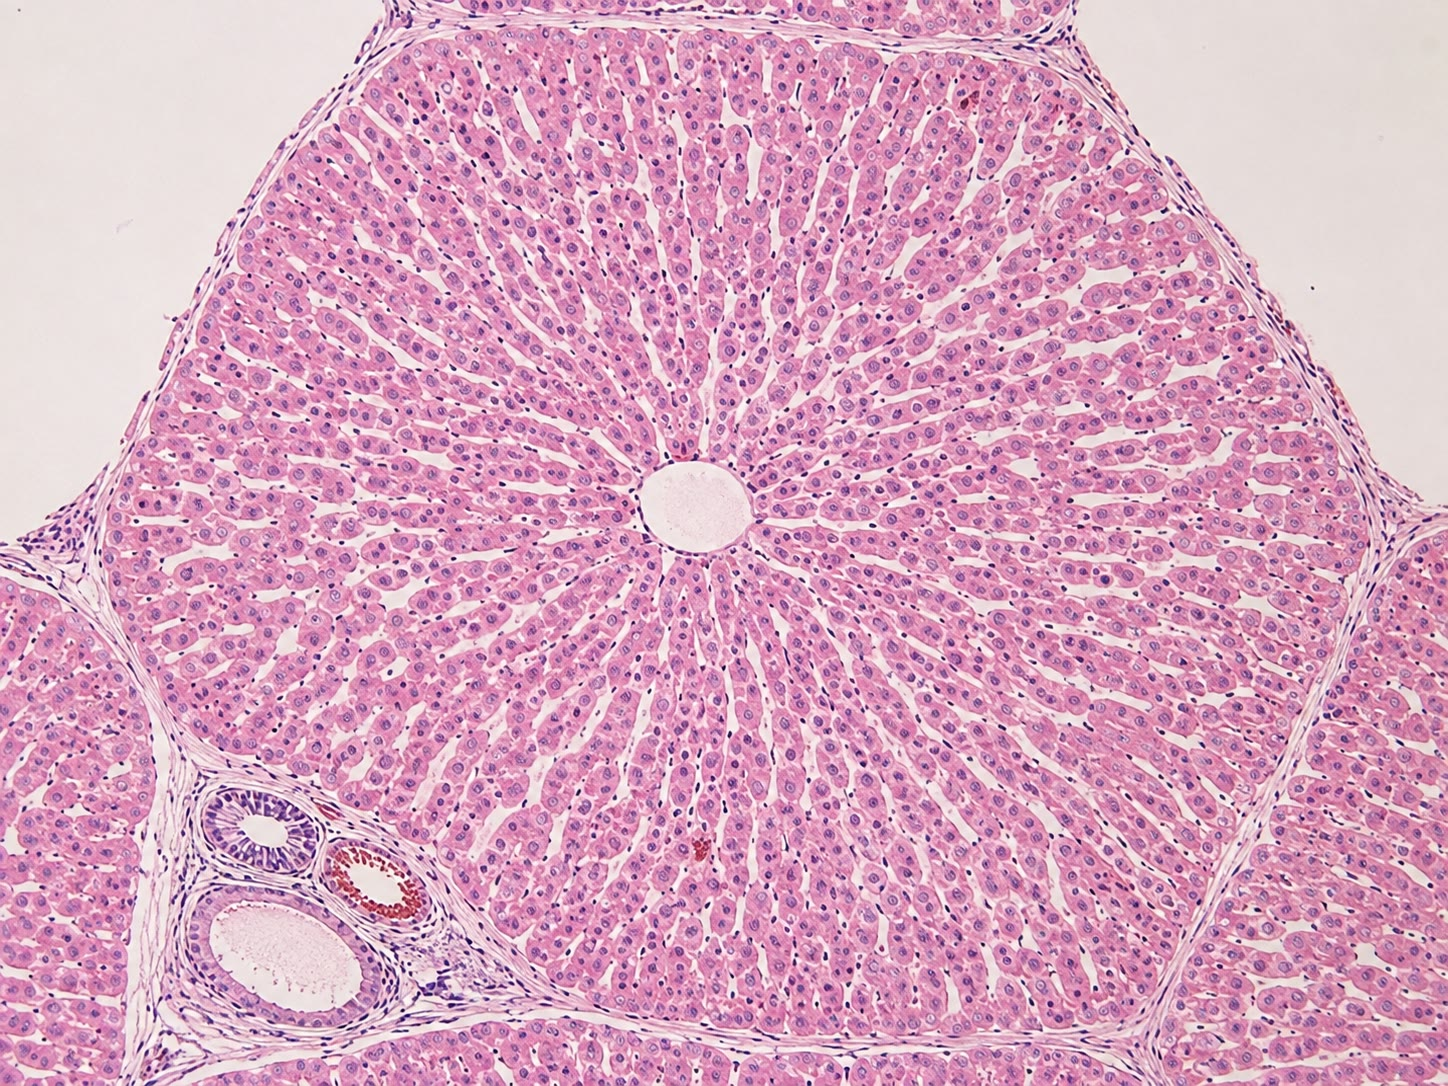
\includegraphics[width=0.52\linewidth]{images/book3/ai/b3-16-liver-lobule-micrograph.jpg}

{\small Un lobulillo hepático: láminas de hepatocitos que irradian desde una
vena central, bañadas por la sangre que llega del tubo digestivo. Estas
\omterm{def:b1:cell-unit-of-life:cell}{células} almacenan \omterm{def:b1:carbohydrates:polysaccharide}{glucógeno}, fabrican glucosa, construyen \omterm{def:b1:lipids:triglyceride}{grasa} y cuerpos
cetónicos y eliminan el nitrógeno: la central metabólica del \omterm{def:b1:organism-environment:organism}{organismo}.}
\end{omfigure}

\begin{method}[Lectura de un estado metabólico]\label{met:b1:biosyntheses-integration:state}
\begin{enumerate}
  \item Pregúntese qué combustible abunda: glucosa alta significa
        almacenamiento (\omterm{def:b1:carbohydrates:polysaccharide}{glucógeno} y después \omterm{def:b1:lipids:triglyceride}{grasa}); glucosa baja significa
        movilización.
  \item Síganse las señales: la insulina activa las sintasas e inactiva la
        fosforilasa y la lipasa; el glucagón hace lo contrario, sobre todo
        por fosforilación de esas mismas \omterm{def:b1:enzymes:enzyme}{enzimas} (\cref{ch:b1:enzymes}).
  \item Compruébense las encrucijadas: el \omterm{def:b1:water-small-molecules:atp}{ATP} y el citrato bloquean la PFK
        y abren la \omterm{def:b1:biosyntheses-integration:gluconeogenesis}{gluconeogénesis}; el AMP hace lo contrario; el
        malonil-CoA bloquea la combustión de \omterm{def:b1:lipids:triglyceride}{grasa} mientras se está
        fabricando \omterm{def:b1:lipids:triglyceride}{grasa}; el \omterm{def:b1:respiration-fermentation:pdh}{acetil-CoA} activa la carboxilasa que inicia la
        \omterm{def:b1:biosyntheses-integration:gluconeogenesis}{gluconeogénesis}.
  \item Asígnense los \omterm{def:b1:mammal-organization:organ}{órganos}: hígado (almacena, fabrica y exporta glucosa;
        fabrica cuerpos cetónicos y urea), músculo (almacena \omterm{def:b1:carbohydrates:polysaccharide}{glucógeno} para
        sí mismo, exporta lactato y alanina), \omterm{def:b1:body-plans-tissues:tissue}{tejido} adiposo (almacena y
        libera \omterm{def:b1:lipids:triglyceride}{grasa}) y encéfalo (quema glucosa y después cuerpos
        cetónicos).
\end{enumerate}
\end{method}

\section{La planta integrada}

\begin{proposition}[Fuente y sumidero]\label{prop:b1:biosyntheses-integration:sourcesink}
De día, los \omterm{def:b1:eukaryotic-cell:plastid}{cloroplastos} de una \omterm{def:b1:flowering-plant-organization:organs}{hoja} exportan triosa fosfato al \omterm{def:b1:eukaryotic-cell:organelle}{citosol},
donde se convierte en \emph{sacarosa} para exportarla por el floema
(\cref{ch:b1:plant-transport}) a las raíces, los frutos y los ápices en
crecimiento; lo que el floema no puede llevarse se guarda en el cloroplasto
como \emph{\omterm{def:b1:carbohydrates:polysaccharide}{almidón}}, una reserva transitoria que se moviliza de noche para
mantener el flujo de sacarosa. Donde el hígado de un mamífero decide entre
\omterm{def:b1:carbohydrates:polysaccharide}{glucógeno} y exportación mediante hormonas, una \omterm{def:b1:flowering-plant-organization:organs}{hoja} decide entre \omterm{def:b1:carbohydrates:polysaccharide}{almidón} y
sacarosa según el nivel de fosfato del \omterm{def:b1:eukaryotic-cell:organelle}{citosol}, que controla el exportador
de la envoltura del cloroplasto. Una planta se regula por las
concentraciones de sus propios metabolitos, \omterm{def:b1:mammal-organization:organ}{órgano} a \omterm{def:b1:mammal-organization:organ}{órgano}; el mamífero
añade un mando nervioso y hormonal sobre el conjunto.
\end{proposition}

\begin{omfigure}
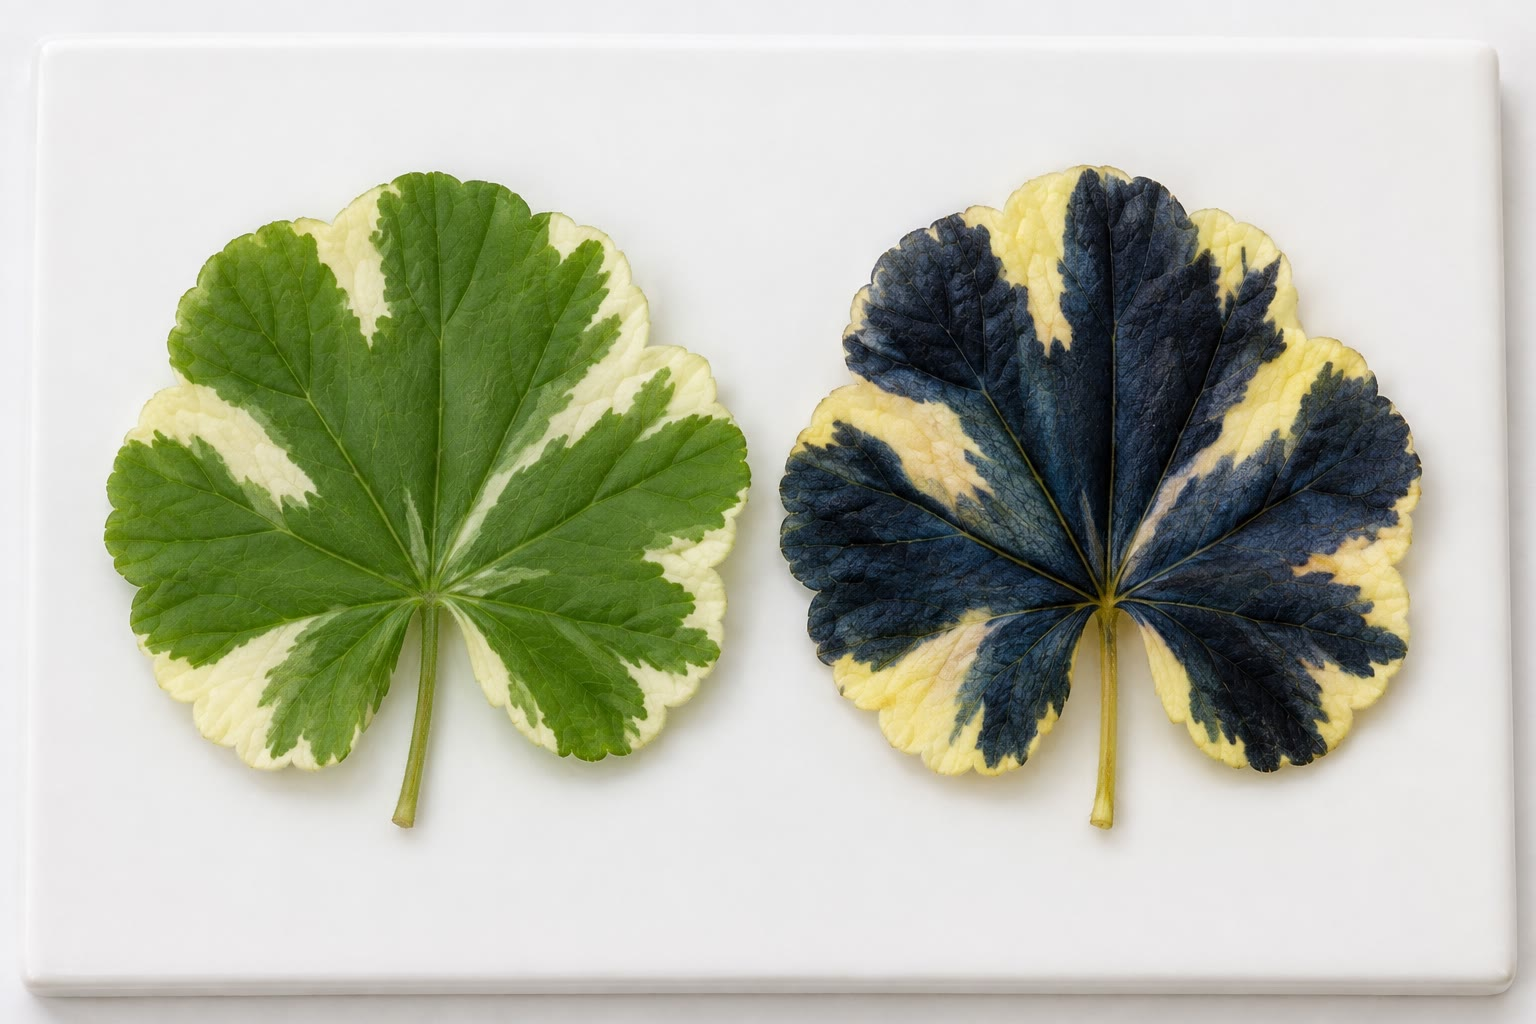
\includegraphics[width=0.6\linewidth]{images/book3/ai/b3-16-variegated-leaf-iodine.jpg}

{\small Una \omterm{def:b1:flowering-plant-organization:organs}{hoja} variegada antes y después de la prueba del yodo: solo se ha
fabricado \omterm{def:b1:carbohydrates:polysaccharide}{almidón} (azul negruzco) allí donde había \omterm{def:b1:photosynthesis:pigments}{clorofila}. Las zonas
blancas, que importaron sacarosa de las verdes, no fabricaron \omterm{def:b1:carbohydrates:polysaccharide}{almidón}
propio.}
\end{omfigure}

\begin{example}[El almidón de una noche]\label{ex:b1:biosyntheses-integration:nightstarch}
Una \omterm{def:b1:flowering-plant-organization:organs}{hoja} aparta como \omterm{def:b1:carbohydrates:polysaccharide}{almidón} alrededor de la mitad de lo que fija durante el
día y lo degrada a un ritmo casi constante a lo largo de la noche, de modo
que la reserva se agota justo antes del alba: si se acorta la noche
artificialmente, sobra \omterm{def:b1:carbohydrates:polysaccharide}{almidón}; si se alarga, la planta pasa hambre en las
últimas horas. El ritmo se ajusta dentro de la primera hora de oscuridad al
tamaño de la reserva y a la duración prevista de la noche: un cálculo hecho
con \omterm{def:b1:enzymes:enzyme}{enzimas} y un reloj, en una \omterm{def:b1:cell-unit-of-life:cell}{célula} sin encéfalo.
\end{example}

\section{Ejercicios}

\begin{exercise}[$\star$]\label{exo:b1:biosyntheses-integration:1}
Nómbrense las tres cosas que necesita una biosíntesis y la vía que
suministra casi todo el \omterm{def:b1:biosyntheses-integration:ppp}{NADPH} de una \omterm{def:b1:cell-unit-of-life:cell}{célula} animal.
\end{exercise}

\begin{exercise}[$\star$]\label{exo:b1:biosyntheses-integration:2}
Enumérense los tres pasos irreversibles de la \omterm{def:b1:respiration-fermentation:glycolysis}{glucólisis} y la \omterm{def:b1:enzymes:enzyme}{enzima} que
esquiva cada uno en la \omterm{def:b1:biosyntheses-integration:gluconeogenesis}{gluconeogénesis}.
\end{exercise}

\begin{exercise}[$\star$]\label{exo:b1:biosyntheses-integration:3}
A partir de la figura de la glucemia, léanse el máximo tras el desayuno, el
tiempo hasta volver a \qty{5}{mmol/L} y el valor mínimo nocturno.
\end{exercise}

\begin{exercise}[$\star$]\label{exo:b1:biosyntheses-integration:4}
¿Por qué una semilla de girasol en germinación puede fabricar azúcar a
partir de su \omterm{def:b1:lipids:triglyceride}{aceite} y un ser humano hambriento no?
\end{exercise}

\begin{exercise}[$\star\star$]\label{exo:b1:biosyntheses-integration:5}
Calcúlense el coste en \omterm{def:b1:water-small-molecules:atp}{ATP} de fabricar una glucosa a partir de dos lactatos
y el coste neto de una vuelta del ciclo de Cori (el músculo gana 2, el
hígado gasta 6). ¿Quién paga, y con qué?
\end{exercise}

\begin{exercise}[$\star\star$]\label{exo:b1:biosyntheses-integration:6}
Un palmitato necesita 8 \omterm{def:b1:respiration-fermentation:pdh}{acetil-CoA}, 7 \omterm{def:b1:water-small-molecules:atp}{ATP} y 14 \omterm{def:b1:biosyntheses-integration:ppp}{NADPH}. ¿Cuántas moléculas de
glucosa deben pasar por la \omterm{def:b1:respiration-fermentation:glycolysis}{glucólisis} y la piruvato deshidrogenasa para
suministrar el \omterm{def:b1:respiration-fermentation:pdh}{acetil-CoA}, y cuántas por la \omterm{def:b1:biosyntheses-integration:ppp}{vía de las pentosas fosfato}
(2 \omterm{def:b1:biosyntheses-integration:ppp}{NADPH} cada una) para suministrar el \omterm{def:b1:biosyntheses-integration:ppp}{NADPH}?
\end{exercise}

\begin{exercise}[$\star\star$]\label{exo:b1:biosyntheses-integration:7}
Explíquese por qué la \omterm{def:b1:biosyntheses-integration:fasynthesis}{síntesis de ácidos grasos} y la $\beta$-oxidación usan
\omterm{def:b1:enzymes:enzyme}{enzimas} distintas, compartimentos distintos y \omterm{def:b1:enzymes:enzyme}{coenzimas} distintas, y cómo
impide el malonil-CoA que funcionen a la vez.
\end{exercise}

\begin{exercise}[$\star\star$]\label{exo:b1:biosyntheses-integration:8}
Escríbase la \omterm{def:b1:biosyntheses-integration:nitrogen}{transaminación} de la alanina con el $\alpha$-cetoglutarato y
nómbrense los productos. ¿En qué sentido transcurre tras una comida rica en
\omterm{def:b1:proteins:peptide}{proteínas}, y en cuál durante un ayuno?
\end{exercise}

\begin{exercise}[$\star\star$]\label{exo:b1:biosyntheses-integration:9}
Un paciente carece de glucosa-6-fosfatasa. Predíganse los efectos sobre la
glucemia entre comidas, sobre el tamaño del hígado y sobre el lactato de la
sangre, con sus razones.
\end{exercise}

\begin{exercise}[$\star\star\star$]\label{exo:b1:biosyntheses-integration:10}
El encéfalo necesita \qty{120}{g} de glucosa al día y \qty{1}{g} de \omterm{def:b1:proteins:peptide}{proteína}
rinde \qty{0.55}{g} de glucosa. Calcúlense la \omterm{def:b1:proteins:peptide}{proteína} que perdería al día
una persona en ayunas para alimentar el encéfalo solo con \omterm{def:b1:biosyntheses-integration:gluconeogenesis}{gluconeogénesis}, y
el músculo que eso representa (\qty{20}{\%} de \omterm{def:b1:proteins:peptide}{proteína}). Explíquese qué
cambian los cuerpos cetónicos si reducen la necesidad de glucosa del
encéfalo a \qty{40}{g}.
\end{exercise}

\begin{exercise}[$\star\star\star$]\label{exo:b1:biosyntheses-integration:11}
La insulina activa la \omterm{def:b1:carbohydrates:polysaccharide}{glucógeno} sintasa e inactiva la \omterm{def:b1:carbohydrates:polysaccharide}{glucógeno} fosforilasa;
el glucagón hace lo contrario. Explíquese por qué ambas no pueden estar
activas a la vez, qué ocurriría si lo estuvieran (calcúlese el \omterm{def:b1:water-small-molecules:atp}{ATP}
desperdiciado por vuelta: un UTP para añadir una glucosa, ninguno para
retirarla), y para qué se usa ese ``ciclo fútil'' en los abejorros que
calientan sus músculos de vuelo.
\end{exercise}

\begin{exercise}[$\star\star\star$]\label{exo:b1:biosyntheses-integration:12}
``Una \omterm{def:b1:cell-unit-of-life:cell}{célula} no tiene plan; tiene válvulas.'' Discútase en un párrafo: el
control alostérico y hormonal de las \omterm{def:b1:enzymes:enzyme}{enzimas} de las encrucijadas, el papel
de tener \omterm{def:b1:enzymes:enzyme}{enzimas} separadas para los sentidos opuestos, y qué emerge de todo
ello que parece un plan.
\end{exercise}

\section{Problema: veinticuatro horas de un ser humano}

\begin{problem}[{Problema de fin de semana --- un día sin desayuno: las
reservas pesadas, el encéfalo alimentado, la proteína contada y la grasa
movilizada, hasta llegar a las horas de ayuno que el glucógeno del hígado
puede cubrir}]
\label{pb:b1:biosyntheses-integration:1}
Un adulto de \qty{70}{kg} gasta \qty{8.4}{MJ} al día (\qty{100}{W} de
media) y contiene: \qty{100}{g} de \omterm{def:b1:carbohydrates:polysaccharide}{glucógeno} hepático, \qty{400}{g} de
\omterm{def:b1:carbohydrates:polysaccharide}{glucógeno} muscular, \qty{12}{kg} de \omterm{def:b1:lipids:triglyceride}{grasa} y \qty{10}{kg} de \omterm{def:b1:proteins:peptide}{proteína} (de la
que \qty{6}{kg} están en el músculo). El encéfalo consume \qty{120}{g} de
glucosa al día (\qty{5}{g/h}); los demás \omterm{def:b1:body-plans-tissues:tissue}{tejidos} dependientes de la glucosa
(glóbulos rojos, médula renal), \qty{40}{g}. Energía: \omterm{def:b1:carbohydrates:monosaccharide}{glúcidos}
\qty{17}{kJ/g}, \omterm{def:b1:lipids:triglyceride}{grasa} \qty{38}{kJ/g}, \omterm{def:b1:proteins:peptide}{proteína} \qty{17}{kJ/g}; \qty{1}{g} de
\omterm{def:b1:proteins:peptide}{proteína} rinde \qty{0.55}{g} de glucosa por \omterm{def:b1:biosyntheses-integration:gluconeogenesis}{gluconeogénesis}, y \qty{1}{g} de
\omterm{def:b1:lipids:triglyceride}{grasa} rinde \qty{0.1}{g} de glucosa (a partir de su glicerol).

\medskip
\noindent\textbf{Parte I --- Las reservas.}
\begin{enumerate}
  \item Calcúlense la energía contenida en cada una de las cuatro reservas,
        en megajulios, y los días de gasto que representa cada una.
  \item ¿Qué reserva puede suministrar glucosa a la sangre directamente?
        ¿Por qué no el \omterm{def:b1:carbohydrates:polysaccharide}{glucógeno} muscular?
  \item Calcúlese la glucosa total que el cuerpo necesita al día para sus
        \omterm{def:b1:body-plans-tissues:tissue}{tejidos} dependientes de la glucosa.
  \item Calcúlense la glucosa de la propia sangre (\qty{5}{mmol/L},
        \qty{5}{L}, \qty{180}{g/mol}) y los minutos que alimentaría al
        encéfalo por sí sola.
  \item ¿Qué fracción del gasto diario es la glucosa del encéfalo?
  \item Tras una comida, el \omterm{def:b1:carbohydrates:polysaccharide}{glucógeno} del hígado está lleno y la glucemia
        sigue subiendo. Nómbrense el siguiente destino de la glucosa y la
        hormona que lo dirige.
\end{enumerate}

\medskip
\noindent\textbf{Parte II --- La noche.}
La última comida termina a las 20:00; a partir de ahí solo el hígado
suministra la glucosa de la sangre.
\begin{enumerate}[resume]
  \item Con \qty{160}{g} de glucosa al día, ¿cuál es la demanda horaria de
        los \omterm{def:b1:body-plans-tissues:tissue}{tejidos} dependientes de la glucosa?
  \item ¿Cuánto duran \qty{100}{g} de \omterm{def:b1:carbohydrates:polysaccharide}{glucógeno} hepático a ese ritmo, si
        nada más suministra glucosa?
  \item En realidad la \omterm{def:b1:biosyntheses-integration:gluconeogenesis}{gluconeogénesis} aporta alrededor de un tercio de la
        glucosa desde las primeras horas. Recalcúlese la duración del
        \omterm{def:b1:carbohydrates:polysaccharide}{glucógeno}.
  \item ¿A qué hora de la mañana se agota el \omterm{def:b1:carbohydrates:polysaccharide}{glucógeno} del hígado según
        cada estimación?
  \item Los músculos, entretanto, queman \omterm{def:b1:lipids:fattyacid}{ácidos grasos}. Calcúlese la \omterm{def:b1:lipids:triglyceride}{grasa}
        oxidada durante la noche (\qty{12}{h}) si les corresponde el
        \qty{60}{\%} del gasto en reposo y solo queman \omterm{def:b1:lipids:triglyceride}{grasa}.
\end{enumerate}

\medskip
\noindent\textbf{Parte III --- El día siguiente, sin comer.}
\begin{enumerate}[resume]
  \item Agotado el \omterm{def:b1:carbohydrates:polysaccharide}{glucógeno}, los \qty{160}{g} de glucosa deben venir de la
        \omterm{def:b1:biosyntheses-integration:gluconeogenesis}{gluconeogénesis}. Calcúlense la \omterm{def:b1:proteins:peptide}{proteína} necesaria al día y la masa
        de músculo que representa.
  \item Calcúlense el \omterm{def:b1:water-small-molecules:atp}{ATP} que el hígado gasta en fabricar \qty{160}{g} de
        glucosa a partir de piruvato (6 \omterm{def:b1:water-small-molecules:atp}{ATP} por glucosa) y su energía a
        \qty{50}{kJ/mol}.
  \item Calcúlese la contribución del glicerol de la \omterm{def:b1:lipids:triglyceride}{grasa}: ¿cuánta \omterm{def:b1:lipids:triglyceride}{grasa}
        se oxida al día si cubre todo el gasto no glucídico, y cuánta
        glucosa rinde su glicerol?
  \item Recalcúlese la \omterm{def:b1:proteins:peptide}{proteína} necesaria restando la contribución del
        glicerol.
  \item A ese ritmo, ¿cuántos días hasta perder la mitad del músculo?
  \item A partir del tercer día el hígado fabrica cuerpos cetónicos y el
        encéfalo toma de ellos dos tercios de su energía; la necesidad de
        glucosa cae a \qty{40}{g} para el encéfalo más \qty{40}{g} para el
        resto. Recalcúlense la pérdida de \omterm{def:b1:proteins:peptide}{proteína} al día y los días hasta
        perder la mitad del músculo.
  \item Calcúlense los días que dura la reserva de \omterm{def:b1:lipids:triglyceride}{grasa} a \qty{8.4}{MJ}
        diarios (que bajan a \qty{6.5}{MJ} en un ayuno prolongado:
        recalcúlese).
  \item Explíquese por qué una persona en ayuno muere por pérdida de
        \omterm{def:b1:proteins:peptide}{proteína} antes de que se agote la \omterm{def:b1:lipids:triglyceride}{grasa}, y qué retrasan los cuerpos
        cetónicos.
\end{enumerate}

\medskip
\noindent\textbf{Parte IV --- Las válvulas.}
\begin{enumerate}[resume]
  \item Nómbrense la \omterm{def:b1:enzymes:enzyme}{enzima} del hígado que debe estar activa a las 03:00 e
        inactiva a las 09:00, y la que debe hacer lo contrario, para el
        \omterm{def:b1:carbohydrates:polysaccharide}{glucógeno}.
  \item Nómbrense la señal (hormona) que las coloca en cada estado y la
        modificación química por la que actúa.
  \item Una \omterm{def:b1:cell-unit-of-life:cell}{célula} hepática a las 03:00 tiene mucho \omterm{def:b1:respiration-fermentation:pdh}{acetil-CoA} procedente
        de la oxidación de \omterm{def:b1:lipids:triglyceride}{grasas}. Nómbrense la \omterm{def:b1:enzymes:enzyme}{enzima} de la
        \omterm{def:b1:biosyntheses-integration:gluconeogenesis}{gluconeogénesis} que eso activa y la \omterm{def:b1:enzymes:enzyme}{enzima} de la \omterm{def:b1:respiration-fermentation:glycolysis}{glucólisis} que el
        \omterm{def:b1:water-small-molecules:atp}{ATP} inhibe al mismo tiempo.
  \item Explíquese por qué la \omterm{def:b1:biosyntheses-integration:gluconeogenesis}{gluconeogénesis} y la \omterm{def:b1:respiration-fermentation:glycolysis}{glucólisis}, funcionando
        a la vez en la misma \omterm{def:b1:cell-unit-of-life:cell}{célula}, solo convertirían \omterm{def:b1:water-small-molecules:atp}{ATP} en calor, y cómo
        lo impiden las \omterm{def:b1:enzymes:enzyme}{enzimas} separadas de los tres desvíos.
  \item Un diabético sin insulina tiene la glucemia alta y, aun así, el
        hígado sigue fabricando glucosa y cuerpos cetónicos. Explíquese la
        paradoja a partir de las válvulas.
  \item Enúnciese el resultado: las horas de ayuno que cubre el \omterm{def:b1:carbohydrates:polysaccharide}{glucógeno}
        del hígado (con y sin \omterm{def:b1:biosyntheses-integration:gluconeogenesis}{gluconeogénesis}), la pérdida diaria de
        \omterm{def:b1:proteins:peptide}{proteína} antes y después del cambio a cuerpos cetónicos, y los días
        que dura la reserva de \omterm{def:b1:lipids:triglyceride}{grasa}.
\end{enumerate}
\end{problem}
